\documentclass[12pt,a4paper]{article}
\usepackage[left=2.5cm,right=2.5cm,top=2.5cm,bottom=2.5cm]{geometry}
\usepackage[utf8]{inputenc}
\usepackage{amssymb, amsmath, amsthm}
\usepackage{graphics, graphicx}
\graphicspath{ {./2.5/} }
\pagestyle{empty}
\newtheorem{lemma}{Lemma}
\newtheorem{thm}{Theorem}

\begin{document}
\textbf{Chapter 2 solutions  \hfill Hanna Gábor}

\begin{enumerate}
  \item
    \textit{In $\epsilon$-greedy action selection, for the case of two actions and $\epsilon = 0.5$, what is the probability that the greedy action is selected?}

    $\mathbb{P}(\text{greedy action is selected}) = 0.5 + 0.5/2 = 0.75.$

  \item
    \textit{Bandit example. Consider a $k$-armed bandit problem with $k = 4$ actions, denoted $1$, $2$, $3$, and $4$. Consider applying to this problem a bandit algorithm using $\epsilon$-greedy action selection, sample-average action-value estimates, and initial estimates of $Q_1(a) = 0$, for all $a$. Suppose the initial sequence of actions and rewards is $A_1 = 1$, $R_1 = 1$, $A_2 = 2$, $R_2 = 1$, $A_3 = 2$, $R_3 = 2$, $A_4 = 2$,
    $R_4 = 2$, $A_5 = 3$, $R_5 = 0$. On some of these time steps the $\epsilon$ case may have occurred, causing an action to be selected at random. On which time steps did this definitely occur? On which time steps could this possibly have occurred?}

    Any action can be an exploratory move.

    What were the greedy options in different time steps?\\
    Step $1$: all actions have $0$ estimated values. Every action is a greedy choice.\\
    Step $2$: $Q_1(1) = 1$. The greedy choice now is $1$. $A_2 = 2$ must have been an\\ explorative move.\\
    Step $3$: $Q_2(2) = 1$. The greedy choice is either $1$ or $2$.\\
    Step $4$: $Q_3(2) = 1.5$. The greedy choice is $2$.\\
    Step $5$: $Q_4(2) = 1.67$. The greedy choice is $2$. $A_5 = 3$ must have been an explorative move.

    On time steps $2$ and $5$ a random action must have been selected.

 \item
    \textit{In the comparison shown in Figure 2.2, which method will perform best in
    the long run in terms of cumulative reward and probability of selecting the best action?
    How much better will it be? Express your answer quantitatively.}

    On the long run, the $\epsilon = 0.01$ method will perform the best in both sense.
    The non-greedy methods will eventually find the best action, but only choose it
    with probability $1 - \epsilon + 0.01 \epsilon $. In the $\epsilon = 0.01$ case this means the method
    chooses the best action with probability $0.991$, while in the $\epsilon = 0.1$ case,
    this probability is $0.91$.

\item
  \textit{If the step-size parameters, $\alpha_n$, are not constant, then the estimate $Q_n$ is
  a weighted average of previously received rewards with a weighting different from that
  given by (2.6). What is the weighting on each prior reward for the general case, analogous
  to (2.6), in terms of the sequence of step-size parameters?}

  \begin{align*}
  Q_{n + 1} = & Q_n + \alpha(R_n - Q_n) = \alpha_n R_n + (1 - \alpha_n)Q_n \\
  = & \alpha_n R_n + (1 - \alpha_n)(Q_{n - 1} + \alpha_{n - 1}(R_{n - 1} - Q_{n - 1})) = \dots \\
  = & \Big(\prod\limits_{j = 1}^n (1 - \alpha_j)\Big) Q_1 +
  \sum\limits_{i = 1}^n \Big(\prod\limits_{j = i + 1}^n (1 - \alpha_j) \Big)\alpha_i R_i \\
  \end{align*}

\item
  \textit{(programming) Design and conduct an experiment to demonstrate the
  difficulties that sample-average methods have for nonstationary problems. Use a modified
  version of the 10-armed testbed in which all the $q_*(a)$ start out equal and then take
  independent random walks (say by adding a normally distributed increment with mean
  zero and standard deviation 0.01 to all the $q_*(a)$ on each step). Prepare plots like
  Figure 2.2 for an action-value method using sample averages, incrementally computed,
  and another action-value method using a constant step-size parameter, $\alpha = 0.1$. Use
  $\epsilon = 0.1$ and longer runs, say of 10,000 steps.}

  \begin{center}
  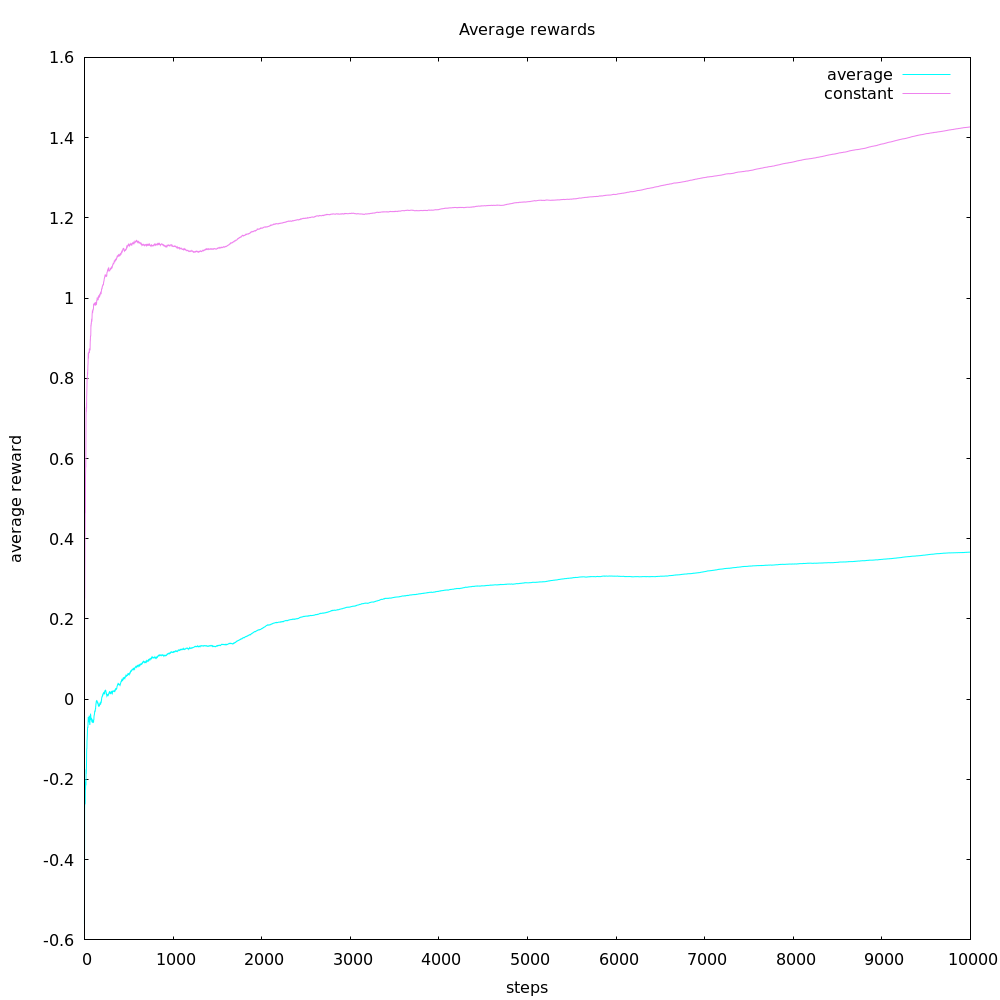
\includegraphics[scale=0.3]{average}
  \\
  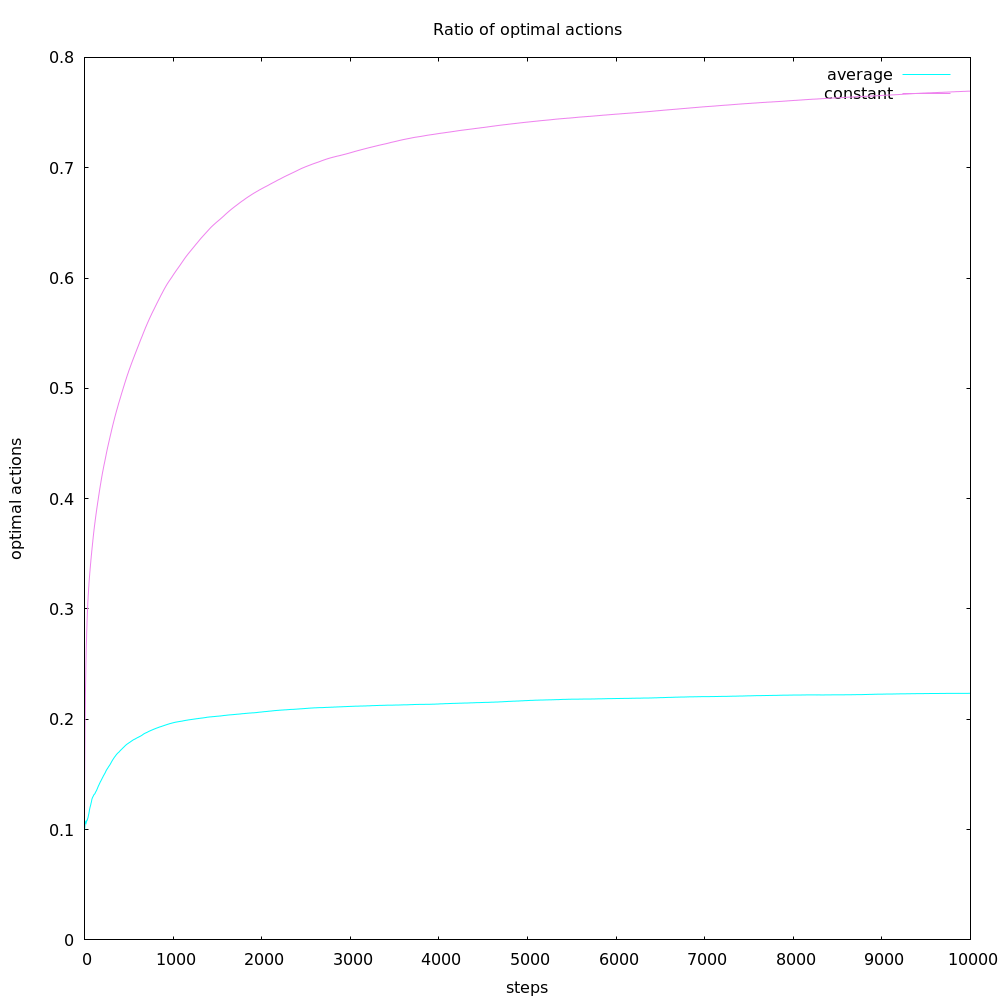
\includegraphics[scale=0.3]{optimal}
\end{center}


\item
  \textit{Mysterious Spikes. The results shown in Figure 2.3 should be quite reliable
  because they are averages over 2000 individual, randomly chosen 10-armed bandit tasks.
  Why, then, are there oscillations and spikes in the early part of the curve for
  the optimistic method? In other words, what might make this method
  perform particularly better or worse, on average, on particular early steps?}

  With very high probability, the first $10$ choices will cover all the possible actions
  once. After the $10^{th}$ action, we have an estimation of the action values based
  on actually trying them, but the optimal starting value still dominates these estimates.
  The $11^{th}$ step is chosen based on the rewards, not on the optimisic starting values,
  this causes a big spike at step $11$. In steps $11-20$ (with high probability) we will
  choose all the actions once, starting with the action that has the highest estimated
  action value and continuing in this order. After $20$ steps, we will have tried all
  the actions twice and at step $21$, we choose an action based on these estimates.
  This will cause a spike at step $21$.
  The starting values will have less and less effect, it won't be true that in steps
  $10k - 10(k + 1)$ we will try all the actions once, so these spikes will disappear.

\item
  \textit{Unbiased Constant-Step-Size Trick. In most of this chapter we have used
  sample averages to estimate action values because sample averages do not produce the
  initial bias that constant step sizes do (see the analysis leading to (2.6)). However, sample
  averages are not a completely satisfactory solution because they may perform poorly
  on nonstationary problems. Is it possible to avoid the bias of constant step sizes while
  retaining their advantages on nonstationary problems? One way is to use a step size of
  \[\beta_n\doteq \alpha / \bar{o}_n\]
  to process the $n^{th}$ reward for a particular action, where $\alpha > 0$ is
  a conventional constant step size, and $\bar{o}_n$ is a trace of one that starts at 0:
  \[\bar{o}_n \doteq \bar{o}_{n - 1} + \alpha(1 - \bar{o}_{n - 1}) \text{ for } n \ge 0 \text{ with } \bar{o}_0 \doteq 0\]
  Carry out an analysis like that in (2.6) to show that $Q_n$ is an exponential recency-weighted
  average without initial bias.
  }
  \begin{align*}
    Q_{n + 1} &= Q_n + \beta_n(R_n - Q_n)\\
    &= \beta_n R_n + (1 - \beta_n)Q_n\\
    &= \beta_n R_n + (1 - \beta_n)(\beta_{n - 1}R_{n - 1} + (1 - \beta_{n - 1}) Q_{n - 1})\\
    &= \beta_n R_n + (1 - \beta_n)\beta_{n - 1}R_{n - 1} + (1 - \beta_n)(1 - \beta_{n - 1}) Q_{n - 1})\\
    &=  Q_1\prod_{i = 1}^n (1 - \beta_i) + \prod_{i = 1} ^n \beta_i \Big(\prod_{j = i + 1}^n (1 - \beta_j)\Big) R_i\\
  \end{align*}
  As $\bar{o}_1 = \bar{o}_0 + \alpha(1 - \bar{o}_0) = 0 + \alpha(1 - 0) = \alpha$ and so
  $1 - \beta_1 = 1 - \alpha/\bar{o}_1 = 1 - \alpha/\alpha = 0$, the coefficient of
  $Q_1$ in the equation above is $0$. That is
    \begin{align*}
    Q_{n + 1} &= \prod_{i = 1} ^n \beta_i \Big(\prod_{j = i + 1}^n (1 - \beta_j)\Big) R_i\\
  \end{align*}

  We can prove by induction that the sum of the coefficients here are $1$, so this is indeed
  a weighted average.

  $\bar{o}_{n + 1}$ is the weighted average of $1$ an $\bar{o}_n.$ This means it increases over time and
  converges to $1$. Because of this, $\beta_n$ starts with value $1$ and converges to $\alpha$.
  Hence, the coefficient of $R_i$ is smaller than $(1 - \alpha)^{n - i}$, hence this is
  recency-weighted average.

\end{enumerate}
\end{document}
